\documentclass[times, utf8, seminar]{fer}
\usepackage{algorithmic}
\usepackage{algorithm}
\usepackage{booktabs}
\usepackage{listings}
\usepackage{xcolor}
\newcommand\myworries[1]{\textcolor{red}{#1}}
\usepackage{hyperref} 
\usepackage{natbib}
\usepackage{subfig}
\usepackage{color}
\usepackage{placeins}
\usepackage{multirow}

\definecolor{mygreen}{rgb}{0,0.6,0}
\definecolor{mygray}{rgb}{0.5,0.5,0.5}
\definecolor{mymauve}{rgb}{0.58,0,0.82}
\renewcommand\labelitemi{•}

\lstset{ %
  backgroundcolor=\color{white},   % choose the background color
  basicstyle=\footnotesize,        % size of fonts used for the code
  breaklines=true,                 % automatic line breaking only at whitespace
  captionpos=b,                    % sets the caption-position to bottom
  commentstyle=\color{mygreen},    % comment style
  escapeinside={\%*}{*)},          % if you want to add LaTeX within your code
  keywordstyle=\color{blue},       % keyword style
  stringstyle=\color{mymauve},     % string literal style
}

\begin{document}

\title{Međujezično prepoznavanje imenovanih entiteta pomoću wikifikacije}

% TODO: Navedite vaše ime i prezime.
\author{Stipan Mikulić}
\voditelj{dr. sc. Jan Šnajder}

\maketitle

\tableofcontents

\chapter{Uvod}
U današnje vrijeme svjedočimo stalni eksponencijali porast svih vrsta podataka, naročito teksta. Zbog tog naglog porasta podataka ljudi više nisu u mogućnosti obraditi te podatke da bi prepoznali bitne i korisne informacije. Riješenje problema krije se u računalnoj obradi podataka. 
Ovim problemom se bavi područje računarske znanosti (engl. computer science), umjetne inteligencije (engl. artificial intelligence) i strojnog učenja (engl. machine learning) koje se naziva obrada prirodnog jezika (engl. natural language processing, NLP). \\
\indent U ovom radu razvit ću model za međujezično prepoznavanje imenovanih entiteta. Za razvoj dobrog modela za klasifikaciju potrebno nam je puno podataka. Prema zadnjim procjenama više od $ 50\% $ sadžaja na internetu je pisano na engleskom jeziku.\footnote{\url{https://en.wikipedia.org/wiki/Languages_used_on_the_Internet}}U potpunoj dominaciji engleskog jezika u svim vrstama podataka i NLP alata i leži motivacija za razvoj međujezičnog modela. \\
\indent Rad je strukturiran tako da u drugom poglavlju opisuje problem, u trećem analizira podatke nad kojima treniramo, validiramo i testiramo model. Četvrto poglavlje opisat će sam model za prepoznavanje imenovanih entiteta, a peto implementciju tog modela. Rezultati i evaluacija će biti opisani u šestom poglavlju. Zadnjem poglavlje će dati kratki zaključak rada.
\chapter{Opis problema}
\citep{Ratinov:2009:DCM:1596374.1596399}
\citep{tjongkimsang2003conll}
\citep{DBLP:conf/conll/TsaiMR16}
\citep{tksintro2002conll}  \\
Prepoznavanje imenovanih entiteta je zadatak ekstrakcije informacija kojem je cilj klasificirati i locirati elemente u predefinirane kategorije kao što su:

\begin{itemize}
	\item Imena -- Osobe, Organizacije, Lokacije
	\item Vremena -- Vrijeme, Datum
	\item Brojevi -- Novac, Postotci
\end{itemize}

Iako su kategorije unaprijed definirane i dalje se postavlja pitanje koliko općenite i obuhvatne trebaju biti. Ovisno o domeni za koju se koriste imenovani entiteti, moguće ih je prizvoljno definirati. Pogledajmo pobliže ovaj problem kroz primjer. Ako sustavu za prepoznavanje imenovanih entiteta damo sljedeći tekst kao ulaz: \\\\
\centerline{Jim  bought 300 shares of Acme Corp. in 2006.}\\\\
na izlazu statava ćemo dobiti:\\\\
\centerline{[Jim]\textsubscript{OSOBA} bought [300]\textsubscript{BROJ} shares of [Acme Corp.]\textsubscript{ORGANIZACIJA} in [2006]\textsubscript{VRIJEME}.}\\\\
U ovom primjeru entitet OSOBA sadrži jedan token dok entitet ORGANIZACIJA sadrži dva tokena.\footnote{\url{https://en.wikipedia.org/wiki/Named-entity_recognition}} U ovom radu želimo prepoznati sljedeće entitete u tekstu:

\begin{itemize}
	\item PER -- Osobe
	\item ORG -- Organizacije
	\item LOC -- Lokacije
	\item MISC -- Razno
\end{itemize}

\chapter{Analiza podataka}
Model za međujezično prepoznavanje imenovanih entiteta razvijen je nad skupovima podataka iz CoNLL02 i CoNLL03 dijeljenog zadatka. Skup podataka uključuje podatke na engleskom, španjolskom i nizozemskom jeziku. CoNLL skup podataka je podskup novinskih članaka Reutersa iz 1996. Entiteti su označeni u 4 razreda: PER, ORG, LOC i MISC. Skup za treniranje su članci iz kolovoza 1996, dok je testni skup iz prosinca 1996. Imenovani entiteti u testnom skupu su znatno različiti od skupa za treniranje što ih čini značajno težim.\citep{Ratinov:2009:DCM:1596374.1596399} \\
\indent Španjolski i nizozemski skup podataka označen je BIO\footnote{Format u kojem se s B (\textbf{B}egining) označavaju riječi na početku entiteta, I (\textbf{I}nside) označavaju riječi unutar entiteta i O (\textbf{O}utside) označavaju riječi koje ne pripadaju ni jednom entitetu.} formatom dok je engleski skup podataka označen IO formatom\footnote{Format u kojem se s I (\textbf{I}nside) označavaju riječi koje pripadaju nekom entitetu i O (\textbf{O}utside) označavaju riječi koje ne pripadaju ni jednom entitetu.} koji sam naknadno pretvorio u BIO.
\begin{center}
\captionof{table}{Broj entiteta u skupovima}
\begin{tabular}{ clcccc }
\hline
language & set & PER & ORG & LOC & MISC \\ \hline
\multirow{3}{*}{eng} & train & 6600 & 6321 & 7140 & 3438 \\
 & validation & 1842 & 1341 & 1837 & 922 \\
 & test & 1617 & 1661 & 1668 & 702 \\ \hline
\multirow{3}{*}{esp} & train & 4321 & 7390 & 4913 & 2173 \\
 & validation & 1222 & 1700 & 984 & 445\\
 & test & 735 & 1400 & 1084  & 339 \\ \hline
\multirow{3}{*}{ned} & train & 4716 & 2082 & 3208 & 3338 \\
 & validation & 703 & 686 & 479 & 748 \\
 & test & 1098 & 882 & 774 & 1187 \\ \hline
\end{tabular}
\end{center}


\begin{center}
  \makebox[\textwidth]{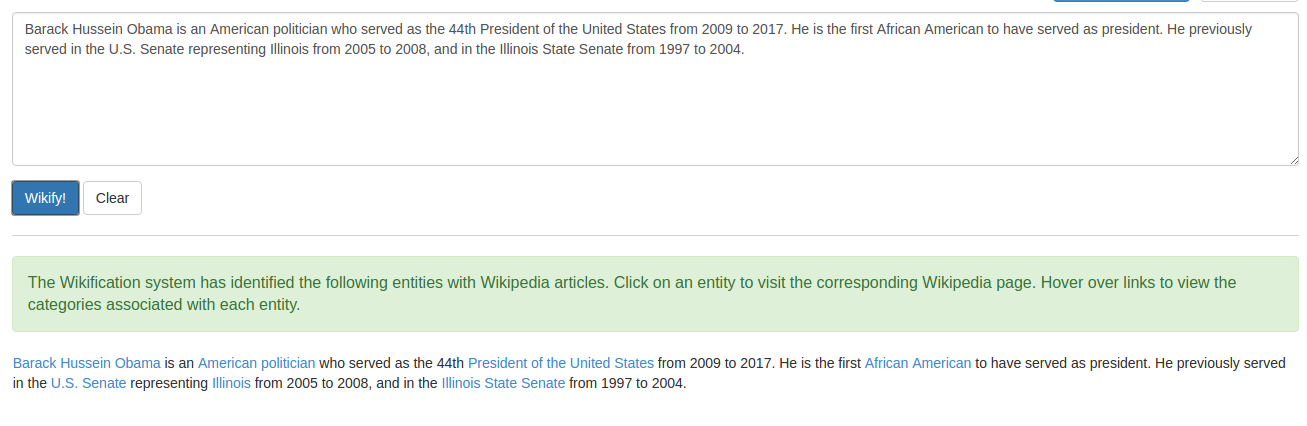
\includegraphics[scale=0.4]{images/eng.png}}
\captionof{figure}{Veličina entiteta skupa podataka na engleskom jeziku}

\end{center}

\begin{center}
  \makebox[\textwidth]{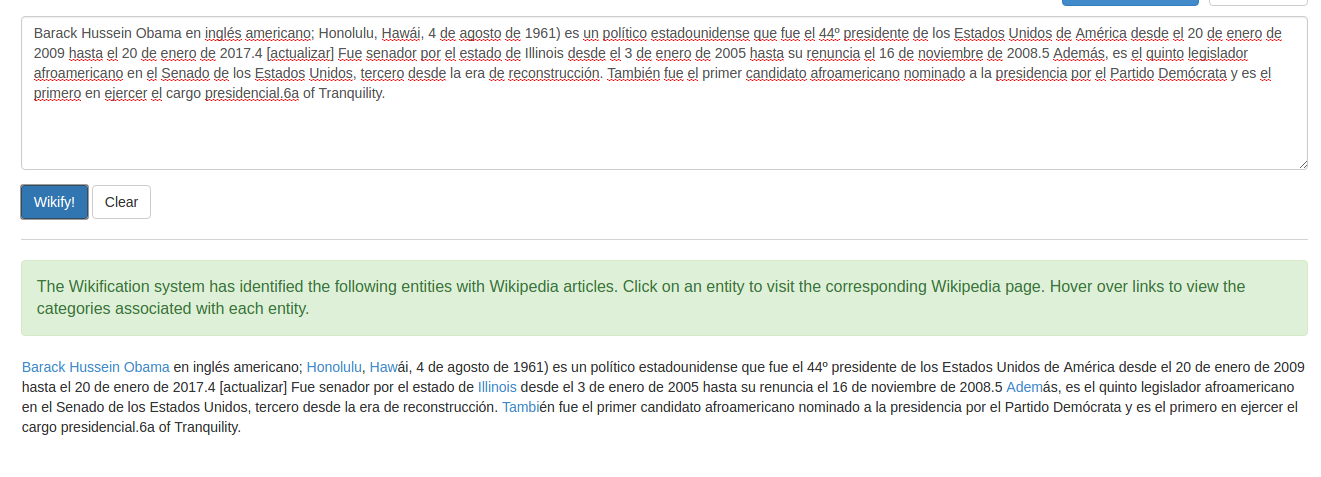
\includegraphics[scale=0.4]{images/esp.png}}
\captionof{figure}{Veličina entiteta skupa podataka na španjolskom jeziku}
\end{center}

\begin{center}
  \makebox[\textwidth]{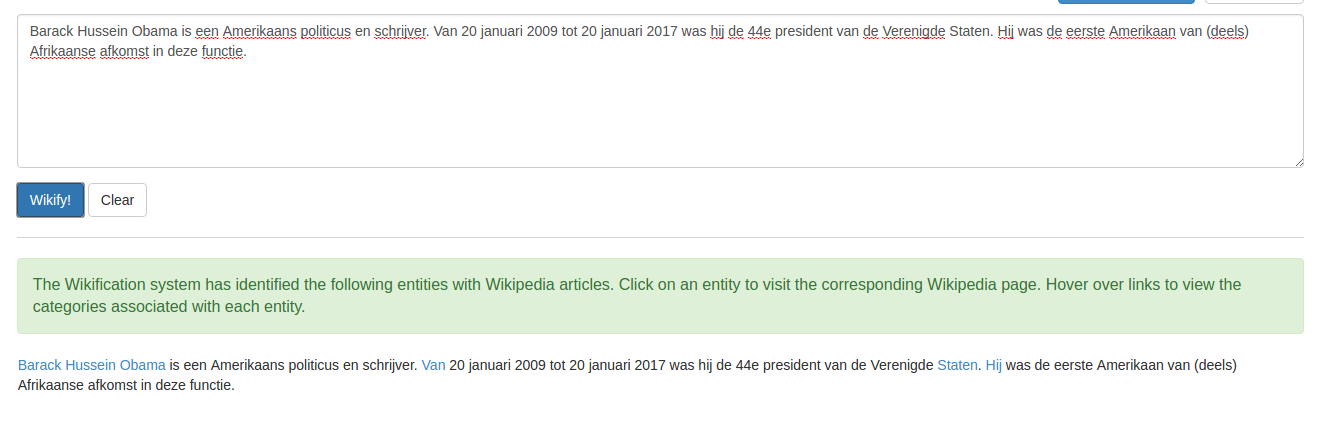
\includegraphics[scale=0.4]{images/ned.png}}
\captionof{figure}{Veličina entiteta skupa podataka na nizozemskom jeziku}
\end{center}
\chapter{Model}

\chapter{Implementacija modela}

\chapter{Evaluacija}

\chapter{Zaključak}

\bibliographystyle{fer}
\bibliography{literatura}
\nocite{*}

\begin{sazetak}


\kljucnerijeci{}
\end{sazetak}
% TODO: Navedite naslov na engleskom jeziku.
\engtitle{Cross-Lingual Named Entity Recognition via Wikification}
\begin{abstract}


\keywords{}
\end{abstract}

\end{document}
